\documentclass[12pt]{article}
%\documentclass[referee]{biom} 
%\usepackage{epsf}
%\usepackage{graphics}
%\usepackage{fullpage}
\usepackage{graphicx}
\usepackage{multirow}
\usepackage{makeidx}
\usepackage{latexsym}
\usepackage{bm}
\usepackage{amsmath}
\usepackage{amsthm}
\usepackage{amssymb}
\usepackage{setspace}

\usepackage{amssymb}
%\usepackage{lscape,rotate}
%\usepackage{rotating}
%\usepackage{xtab}
\usepackage{graphicx}
\usepackage{multirow}
\usepackage{makeidx}
\usepackage{latexsym}
\usepackage{bm}
\usepackage{amsmath}
\usepackage{amsthm}
\usepackage{amssymb}
\usepackage{setspace}
%\usepackage{rotating}
%\usepackage{tabularx}
%\usepackage{booktabs}

 
%\onehalfspacing
\doublespacing
\setlength{\textheight}{22.5cm}
\setlength{\textwidth}{6.47in}
\setlength{\oddsidemargin}{-1mm}
\setlength{\topmargin}{0.1cm}
\setlength{\evensidemargin}{-5mm}
\makeindex

\newcommand{\captionfonts}{\footnotesize}
\makeatletter  
\long\def\@makecaption#1#2{
  \vskip\abovecaptionskip
  \sbox\@tempboxa{{\captionfonts #1: #2}}
  \ifdim \wd\@tempboxa >\hsize
    {\captionfonts #1: #2\par}
  \else
    \hbox to\hsize{\hfil\box\@tempboxa\hfil}
  \fi
  \vskip\belowcaptionskip}
\makeatother


\newcommand {\hide}[1] {\typeout{ #1 }}
\newcommand{\beq}{\begin{equation}}
\newcommand{\eeq}{\end{equation}}
\newcommand{\dif}[2]{\frac{{\rm d} #1}{{\rm d} #2}}
\newcommand{\ildif}[2]{{\rm d} #1/{{\rm d} #2 }}
\newcommand{\ilpdif}[2]{\partial #1/{\partial #2 }}
\newcommand{\pdif}[2]{\frac{\partial #1}{\partial #2}}
\newcommand{\pddif}[3]{\frac{\partial^2 #1}{\partial #2 \partial #3}}
\newcommand{\ilpddif}[3]{\partial^2 #1/{\partial #2 \partial #3}}
\newcommand{\comb}[2]{\left (\begin{array}{c}{#1}\\{#2}\end{array}\right )}
\newcommand{\perm}[2]{^{#1}{\rm P}_{#2}}
\newcommand{\gfrac}[2]{\mbox{$ { \textstyle{ \frac{#1}{#2} }\displaystyle}$}}
\newcommand{\defn}{\begin{quote}{\bf Definition. }}
\newcommand{\edefn}{\end{quote}}
\newcommand{\thm}{\begin{theorem}}
\newcommand{\ethm}{\end{theorem}}
\newcommand{\R}{{\sf R}}
\newcommand{\s}{{\sf S}}
\newcommand{\fnzero}{\setcounter{footnote}{0}}
\newcommand{\bmat}[1]{\left ( \begin{array}{#1}}
\newcommand{\emat}{\end{array}\right )}
\newcommand{\E}{\mathbb{E}}
\newcommand{\ts}{^{\sf T}} 
\newcommand{\its}{^{\sf -T}}
\newcommand{\fv}{\hat{\bm{\mu}}}
\newcommand{\X}{{\bf X}}
\newcommand{\Xt}{\X\ts}
\newcommand{\y}{{\bf y}}
\newcommand{\A}{{\bf A}}
\newcommand{\Qf}{{\bf Q}_{\rm f}}
\newcommand{\bp}{{\bm \beta}}
\newcommand{\rsd}{\hat {\bm \epsilon}}
\newcommand{\grad}{\nabla_\beta}
\newcommand{\tr}[1]{{\rm tr}\left ( {#1} \right )}
\theoremstyle{definition}
\newtheorem*{defin}{Definition}
\theoremstyle{plain}
\newtheorem{theorem}{Theorem}
\newcommand{\rss}{{\cal S}}
\newcommand{\eps}[3]
{{\begin{center}
\rotatebox{#1}{\scalebox{#2}{\includegraphics{#3}}}
\end{center}}
}
\newcommand{\smsz}{\small}


\begin{document}


\title{Modeling the Spatiotemporal Distribution of the Incidence of Resident Foreign Population in Italy}

\author{
Giampiero Marra \\ \small Department of Statistical Science, University College London \\ \small Gower Street, London WC1E 6BT, U.K. \\ \small \texttt{giampiero@stats.ucl.ac.uk}
 \and
David L. Miller \\ \small Department of Mathematical Sciences, University of Bath \\ \small Claverton Down, Bath BA2 7AY, U.K.
 \and
Luca Zanin \\ \small Department of Analysis and Economic Research, Prometeia \\ \small G. Marconi, Bologna 40122, Italy
}

\maketitle


\begin{abstract}

Recently, many European countries have experienced a substantial increase in the proportion of immigrants in the population. The incidence of resident foreigners calculated on a national level does not provide information on the spatial and temporal distribution of the phenomenon, which may be crucial to demographers, economists, sociologists, and policy makers (to name a few) to study and formulate adequate policies supporting, e.g., the process of integration of resident foreigners in a host country. In this paper we suggest a tool for practitioners to provide spatiotemporal maps representing, in space, the distribution of the incidence of resident foreigners in the territory, and over time, changes in spatial trends. In doing this, we use Italian data at municipal level, for the period 2003-2008. The temporal trend of the incidence occurs at different strengths and patterns depending on the spatial location hence it is necessary to allow for such interaction in the model. We propose using a generalized additive model incorporating a scale-invariant smoother of the time and space dimensions. Specifically, we set up a tensor product smooth combining a cubic regression spline basis for time and a soap film spline basis for space. In addition, we construct a composite indicator representing economic and labor market factors to explain some of the observed spatial heterogeneity. The employed approach provides a consistent framework to produce spatiotemporal maps which could be effectively used by policy makers to decide the allocation of economic resources at local level.

\vspace{0.4cm}
\noindent \textbf{Key Words:} Composite indicator; Generalized additive model; Incidence of resident foreigners; Policy-making; Soap film spline basis; Spatiotemporal maps; Tensor product smooth. 


\end{abstract}

\section{Introduction \label{IN}}
Increased political interest as well as academic interest has led to a large amount of research into international migration, both theoretical and empirical, exploring its causes and consequences. Several theories of migration have been proposed, from both a macro- and microeconomic point of view, based on different schools of thought. Among these are the neoclassical economic theory (e.g., Borjas 1989; Massey et al. 1993), the assumptions regarding the new economics of migration (e.g., Stark and Bloom 1985; Massey et al. 1993), dual labor markets (e.g., Piore 1979; Massey et al. 1993) and world systems theory (e.g., Wallerstein 1974; Hooghe et al. 2008). In addition to theoretical work, many empirical studies have taken place. Examples include studies investigating: the impact of resident foreigners on the labor market of the host country (e.g., Borjas 2003, 2005; Borjas, Freeman and Katz 1996; Card 2005; Fullin and Reyneri 2010), underemployment (Slack and Jensen 2007), possible connections between immigration and nations' poverty rates (Raphael and Smolensky 2009), transfer of identity from the first to second generation immigrants (Casey and Dustmann 2010), difference in education, earnings and employment between first and second generation immigrants (Algan et al. 2010), problems relating to the integration of different cultures and languages (e.g., Lazear 1999; Contucci and Ghirlanda 2007), and the tendency for immigrants to live in ethnic ``enclaves'' (Edin, Fredriksson and Aslund 2003). 
  
Manning (2010) has pointed out that many European countries have recently experienced a substantial increase in the proportion of immigrants in the population. Given a specific area such as municipality, province, region, or nation, a measure of density of resident foreign population is the percentage incidence of resident foreigners (IRF), given as the ratio of the number of resident foreigners to the total resident population multiplied by 100 (e.g., Lowell 2007; Coleman 2008; Miguet 2008). This gives a simple, well-known, demographic indicator for comparing different regions of a country in terms of number of resident foreigners per 100 resident inhabitants (e.g., OECD 2004). 

Here we consider the Italian case. According to the Italian National Statistical Office (ISTAT), the IRF has grown substantially, from 2.7\% in 2002 to 6.5\% in 2008. This phenomenon has had an impact on the population, especially from a socio-demographic point of view (see Section \ref{DEM} for details). The IRF calculated on a national level does not tell us anything specific on the spatial distribution of the phenomenon. In order to study and formulate adequate policies supporting, e.g., the process of integration of resident foreigners in a host country, demographers, economists, sociologists, and policy makers should find information on how the distribution of the IRF changes over time and space useful.

To the best of our knowledge, no studies have attempted to model the spatiotemporal distribution of the IRF in a country. Our study uses annual Italian data for the period 2003-2008. Since 2003, ISTAT has provided a new public database with annual frequency of the number of resident foreigners at a municipal level. This represents the current maximum spatial and temporal detail available. Our emphasis is to suggest a tool for practitioners to provide spatiotemporal maps representing, in space, the distribution of the IRF in the territory, and over time, changes of spatial trends. The results of such an investigation complement previous findings in the literature.

To assess what draws resident foreigners to one particular area over another, it is useful to have some quantitative measure of the ``attractiveness'' of each area to resident foreigners. Here, we focus on economic and labor market factors, construct a composite indicator that we have named `Indicator of Spatial Economic Attractiveness' (ISEA) and produce spatiotemporal maps of this. Three important variables constitute the composite indicator: (i) added value per capita at constant price (base year 2000), (ii) unemployment rate and (iii) employment rate. Since these are typically readily available, this composite indicator can be easily constructed for many countries. The results can be analyzed in the light of the spatiotemporal maps of the IRF.

A number of methodologies have been proposed for space-time modeling (see, e.g., Augustin et al. (2009) and references therein). We opt for the spline approach to perform smoothing over some bounded domain $\Omega\subseteq\mathbb{R}^2$, over time (e.g., Hastie and Tibshirani 1990; Ruppert, Wand, and Carroll 2003; Wood 2006). Because currently no relevant economic data are available at municipal level, the response (IRF) is only modeled as a smooth function of time and spatial coordinates. The model is then used to create smooth maps of the geographical area of interest over time. Two points are noteworthy here. First, when a geographical region has complex boundaries, as in many applied contexts, features from one part of the domain can unduly influence other parts giving rise to a phenomenon known as \textit{leakage} (e.g., Ramsay 2002). Leakage typically occurs when a smoother inappropriately links two parts of a domain causing the fitted surface to be mis-estimated, leading to incorrect inference (e.g., biased incidence estimates), which is clearly not desirable. This issue can be overcome if the smoother used can account for the structure of the domain that is under investigation; several solutions have been proposed (e.g., Ramsay 2002; Wood, Bravington and Hedley 2008, and references therein). Second, because it is unlikely that the IRF occurs at similar strengths and patterns over the territory, the employed approach should account for a space-time interaction. These two goals can be jointly achieved by using a scale-invariant three-dimensional tensor product smoother combining a cubic regression spline basis function for time trend and a soap film spline basis for the spatial dimensions (Wood 2006; Wood, Bravington and Hedley 2008).

%\section{Data \label{DAT}}

\section{The structure and nature of the data on resident foreign population \label{SDC}}

The entry of foreigners from some countries of the European Union (EU) into Italy is regulated by the Schengen agreements. These allow for the elimination of border controls, hence creating a common area of free movement among the State members (Broeders 2007). Foreigners from a non-EU country must possess a visa or the necessary documents (further are available from the Ministry of the Interior http://www.interno.it). 
 
In studying a phenomenon linked to the international migration, it is important to distinguish between those individuals considered to be the resident foreign and those considered to be immigrants. The resident foreign population includes all people (born in Italy or abroad) who declare their citizenship to not be Italian. The immigrant population consists of all those born abroad who have declared themselves to be foreigners or Italian by naturalization. Foreigners born in Italy such as children born from foreign parents are excluded from immigrant population. The population census conducted by ISTAT in 2001 showed that foreigners and immigrants constitute roughly the same group: about $81\%$ of immigrants have been identified by foreign citizenship, and $88\%$ of foreigners are immigrants (since they were born abroad).

In many countries, official statistics report the number of resident foreigners, but not the number of immigrants (Coleman 2008). Currently, the dynamics of immigration to Italy still allow the acceptance of a definition which does not distinguish between these two groups. This simplification is reasonable during the first phase of the immigration process in a country, and when the majority of immigrants keep their own citizenship for a long period. Indeed, this is the case in Italy. The population census gives the best distinction between immigrants and foreigners. In this case the data can be analysed by birthplace, citizenship at birth, and citizenship at the census time. 
 
Italian official statistics on the resident foreign population are mainly based on administrative sources linked to specific laws. Recently ISTAT has integrated the official statistics with a new public database (http://demo.istat.it). The database gives the number of resident foreigners calculated at the end of December each year in each municipality (of which there are around 8100). Compared to provincial or regional data, municipal-level data offers far more detail on the spatial distribution of the IRF in the total population.
 
Populations are dynamic over time as well as space. In this regard, the change in number of resident foreign people at municipal level, at the end of a year, is determined by
$$
\text{RFP}^{31^\text{th}} = \text{RFP}^{1^\text{st}} + (I_1 + I_2 + I_3+ I_4) - (D_1 + D_2 + D_3 + D_4 + AC).
$$ 
$\text{RFP}^{31^\text{th}}$ indicates the total number of resident foreigners at the end of December, and $\text{RFP}^{1^\text{st}}$ the number of resident foreigners on the $1^\text{st}$ of January. $I_{1}$ denotes the number of people whose parents are foreigners (at least one of them being resident in the municipality), $I_{2}$ the number of foreign citizens who asked to transfer their residence from another Italian municipality to the current one, $I_{3}$ those who asked to transfer their residence from abroad, and $I_{4}$ refers to recording operations due to other reasons (e.g., foreigners mistakenly deleted from the registry of the municipality, because they were temporarily missing). $D_{1}$ represents the number of resident foreigners who died during the year, $D_{2}$ those who moved to a different municipality, $D_{3}$ those who moved abroad, $D_{4}$ refers to cancellations for other reasons (e.g., foreigners deleted from the registry of the municipality, because they were not present), and \textit{AC} denotes those resident foreigners who obtained Italian citizenship during the year. 

Acquisition of Italian citizenship by foreigners is regulated by law 91 of the $5^\text{th}$ of February 1992 and its subsequent amendments and additions. Foreigners can acquire the Italian citizenship by marriage to an Italian or by naturalization. The latter case refers to the situation in which the foreigner has lived in the country from a certain period of time. Such a period varies dependent on the status of the person in question and the specific laws of each country. For example, in Italy, the period is at least 10 years for non-EU citizens, at least 4 years for EU citizens and at least 5 years for political refugees or stateless persons and adult individuals who been adopted by Italian citizens. An exhaustive list of ways to obtain Italian citizenship is available on the Ministry of the Interior's website. Once foreigners have acquired Italian citizenship, they are included in the Italian population's statistics. Hence, these individuals will come out from the numerator of the IRF. However, our aim is to investigate and measure the incidence on the population of  residents who have not the Italian citizenship.

We do not tackle the issue of illegal foreigners presents in the country. This phenomenon and its respective quantification is an open topic of discussion in the studies of international migrations (e.g., Carter 1999; Hillman and Weiss 1999; Cangiano 2008; Strozza 2004). Several approaches have been proposed in literature to quantify this, but all are subject to criticism (especially with regard to the magnitude of errors in the estimates). Here we only consider official data on the resident foreign population. 

\section{The resident foreign population's contribution to Italy's demography \label{DEM}}

Bijak et al. (2007) shows that in the absence of migration, many of the 27 European Union countries could see a decline in their non-immigrant populations up to 2052. In particular, with no migration they estimate that the population of Italy could decrease from 57 million in 2002 to about 43 million in 2052. The main causes of this decline may be linked to a low fertility rate and hence an aging population. 

Looking at a traditional indicator that describes the weight of the elderly population, the ratio of old (over 64) to young (up to 14) in the total population was 143.4\% at the end of 2008 (156.2\% if we only consider individuals with Italian citizenship). The elderly population is about $43\%$ larger than the young population. Considering only the resident foreign population the ratio is 11.2\%. In the same year, the average age of foreigners resident in Italy was 31, while that of Italian citizens was 43. From this information we can see that if we stratify by citizenship there is a substantial difference in the age structure of the population present in Italy.

As for the low fertility rate, the latest data from ISTAT puts the average number of children per Italian women of childbearing age (from 15 to 49 years) at 1.33, lower than the average of 2.05 children for foreign women living in Italy. Combining the fertility rate for both Italian and foreign women, we obtain an average of 1.41. Coleman (2008) states that ``typically, in low-mortality populations a total fertility of about 2.04 is regarded as the `replacement level', that is, a level sufficient to replace the population in the long-run, ignoring migration''. Given the impact of resident foreigners on the population structure, the measure of total fertility (and hence the level of replacement) must take into account the contribution of immigrants (Coleman 2008). The increasing presence of resident foreigners over recent years has contributed not only to population growth, but also to a reduction in average age and an increase in the total fertility rate. The profile of the nationalities of resident foreigners in Italy is changing. Based on elaborations of data from ISTAT, in 2003, the top three countries represented were Albania (13.6\%), Morocco (12.7\%) and Romania (8.9\%). In 2008, Romania was top (20.5\%), followed by Albania (11.3\%) and Morocco (10.4\%). The significant increase of the Romanian population in Italy coincides with the country's entry to the European Union ($1^\text{st}$ January 2007). Currently, Romanian is the most numerous foreign nationality in 14 of the 20 Italian regions. Italy hosts the largest Romanian community outside Romania and almost half of the entire Romanian migrant stock. The choice of Italy as primary destination for Romanians can be explained by many factors including the presence of small Italian companies, the economic links with Romania, and the accessibility of the Italian language for Romanians (Ban 2009). 

According to a descriptive analysis of ISTAT data, in 2008 the resident foreign population in Italy was made up of 53.6\% individuals from Europe, 22.4\% from Africa, 15.8\% from Asia, 8.1\% from America, and 0.1\% from Oceania.

\section{Spatiotemporal modeling \label{METH}}

\subsection{Model specification \label{MS}}

The model we employ belongs to the class of generalized additive models (GAMs, Hastie and Tibshirani 1990). Such models allow for complex, non-linear relationships between covariates and the response, which can be crucial to uncover interesting features in the data. The IRF exhibits a positive continuous distribution. The proposed model is as follows
\beq
\text{log}\left\{\E(\texttt{irf}_{it})\right\} = f(\texttt{year}_t,\texttt{n}_i,\texttt{e}_i), \ \texttt{irf}_{it} \sim \text{Tweedie}\left(\E(\texttt{irf}_{it}),\phi \E(\texttt{irf}_{it})^{p}\right),          
\label{PropM}
\eeq
at municipality $i=1,\ldots,8094$ and year $t=2003,\ldots,2008$. $\phi$ is a dispersion parameter and the log link function ensures positive fitted values. $\texttt{irf}_{it}$, $\texttt{n}_i$, and $\texttt{e}_i$ represent the variables percentage IRF, Northing, and Easting, respectively. Tweedie distributions are a special case of an exponential dispersion model and include, for example, the normal ($p=0$), Poisson ($p=1$) and gamma ($p=2$) distributions (e.g., J\o rgensen 1987). For $1<p<2$ Tweedie distributions can be represented as Poisson mixtures of gamma distributions, with mass at zero but otherwise continuous on the positive reals. These are especially appealing for modeling continuous positive observations when exact zeros occur. Dunn and Smyth (2005) provided a survey of published applications stressing the usefulness and flexibility of this class of distributions. The function $f$ is a multidimensional smooth of \texttt{year}, \texttt{n}, and \texttt{e} which models the joint effect of these variables on \texttt{irf}. The use of a three-dimensional smoother for time and space is crucial in that the temporal trend of the IRF is expected to occur at different strengths and patterns depending on the spatial location, because of differing site characteristics in the territory. Northing and Easting are simply offsets in kilometers from a set point, thus ensuring that the spatial part of the smooth is isotropic (as opposed to using latitude and longitude). We want both the time and space dimension to have an optimal degree of smoothness in terms of the bias-variance trade-off; the chosen smoother has to be invariant to the relative scaling of space (km) and time (years). In addition, the smoother has to allow for combinations of different basis functions most suitable for the time and space dimensions. This can be achieved by using a multidimensional tensor product smooth combining a cubic regression spline basis for \texttt{year} and a soap film spline basis for the two spatial dimensions \texttt{n} and \texttt{e}; thus accounting for the structure of the geographical domain under investigation (details are given in the next two sections). The smooth component in (\ref{PropM}) is subject to some identifiability constraint; see Wood (2006) for more details.

The next two sections cover the technical details of the construction of the smoothers. We first show how, in general a three-dimensional tensor product smoother can be constructed using a one-dimensional temporal smoother and a two-dimensional spatial smoother. We then go into the details of the construction of the two-dimensional smoother.

\subsection{A three-dimensional tensor product smoother for time and space \label{3D}}

The construction of a three-dimensional scale invariant tensor product smoother of time and space is based on a marginal one-dimensional spline basis for time and a two-dimensional marginal smooth for space, with associated quadratic penalties measuring their roughness. We omit the subscripts $i$ and $t$ for simplicity. Let us assume that we have two low-rank regression spline bases of any type to represent the smooth functions $f_\text{year}$ and $f_\text{space}$, we can write (e.g., Ruppert, Wand and Carroll 2003; Wood 2006)
$$
f_\text{year}(\texttt{year})=\sum_{l=1}^L \xi_l b_l(\texttt{year})=\textbf{X}_\text{year}\bm\xi \ \ \text{and} \ \ f_\text{space}(\texttt{n},\texttt{e})=\sum_{r=1}^R \varphi_r d_r(\texttt{n},\texttt{e})=\textbf{X}_\text{space}\bm\varphi,
$$
where the $b_l(\texttt{year})$ and $d_r(\texttt{n},\texttt{e})$ are known cubic regression spline and soap film basis functions, with corresponding parameters $\xi_l$ and $\varphi_r$ and spline dimensions $L$ and $R$. $\textbf{X}_\text{year}$ and $\textbf{X}_\text{space}$ are marginal model matrices evaluating the basis functions with parameter vectors $\bm\xi$ and $\bm\varphi$. The expansion for $f_\text{space}$ and its roughness penalty do not correspond exactly to the expressions used to set up the model since, in this section, we are concerned with illustrating the construction of a three-dimensional scale invariant tensor product smoother. It is therefore convenient to keep the description of the two-dimensional marginal smooth for space and its quadratic penalty as simple as possible; a rigorous description will be given in the next section. 

In order to set up a three-dimensional tensor product smoother for time and space we need $f_\text{year}(\texttt{year})$ to vary smoothly within the space dimensions. This can be achieved by allowing the parameters $\xi_l$ to vary smoothly with \texttt{n} and \texttt{e}. Using the spline set-up for $f_\text{space}(\texttt{n},\texttt{e})$ we may write (e.g., Wood 2006, p. 163)
$$
\xi_l(\texttt{n},\texttt{e})=\sum_{r=1}^R \varphi_{lr} d_r(\texttt{n},\texttt{e})
$$    
which results in
$$
f(\texttt{year},\texttt{n},\texttt{e})=\sum_{l=1}^L \sum_{r=1}^R \varphi_{lr} d_r(\texttt{n},\texttt{e}) b_l(\texttt{year}). 
$$
For any particular set of observations of \texttt{year}, \texttt{n}, and \texttt{e}, there exists a simple relationship between the matrix $\textbf{X}$ evaluating the tensor product smooth at these observations, and the model matrices $\textbf{X}_\text{year}$ and $\textbf{X}_\text{space}$ evaluating the marginal smooths at the same observations. Ordering appropriately the parameters $\varphi_{lr}$ into a vector $\bm\theta$, the $i^{th}$ row of $\textbf{X}$ is given by $\textbf{X}_{i}=\textbf{X}_\text{year,i}\otimes\textbf{X}_\text{space,i}$, where $\otimes$ is the Kronecker product. 

In the GAM context, it is necessary to quantify the roughness of the smooth functions in the model so that over-fitting can be accounted for and hence avoided during the parameter estimation process (e.g., Marra and Radice 2010). As for the penalty associated with this tensor product basis, it is possible to start from roughness measures associated with the marginal smooths $f_\text{year}(\texttt{year})$ and $f_\text{space}(\texttt{n},\texttt{e})$. Suppose that functionals $Js$ measuring the roughness of the smooth terms are available, and that these can be written as quadratic forms in the marginal parameters, we have that
$$
J_\text{year}(f_\text{year})=\bm\xi\ts\textbf{S}_\text{year}\bm\xi \ \ \text{and} \ \ J_\text{space}(f_\text{space})=\bm\varphi\ts\textbf{S}_\text{space}\bm\varphi,
$$
where the $\textbf{S}$ matrices contain known coefficients whose values depend on the chosen bases for time and space. For instance, the second-order cubic spline penalty for $f_\text{year}(\texttt{year})$ evaluates $J_\text{year}(f_\text{year})=\int\left( \partial^2 f_\text{year}/\partial \texttt{year}^2 \right)^2 \text{d}\texttt{year}$, but it may be more complex (Wood 2006, 2008). Following, e.g., Augustin (2009), an overall penalty for the tensor product smooth can be obtained by applying the penalties of $f_\text{space}(\texttt{n},\texttt{e})$ to the varying coefficients of the marginal smooth $f_\text{year}(\texttt{year})$, $\xi_l(\texttt{n},\texttt{e})$,
$$
\sum_{l=1}^L J_\text{space}\left\{  \xi_l(\texttt{n},\texttt{e}) \right\},
$$ 
and the penalties of $f_\text{year}(\texttt{year})$ to the varying coefficients of the marginal smooth $f_\text{space}(\texttt{n},\texttt{e})$, $\varphi_r(\texttt{year})$,  
$$
\sum_{r=1}^R J_\text{year}\left\{  \varphi_r(\texttt{year}) \right\}.
$$ 
It follows that the roughness penalty of $f(\texttt{year},\texttt{n},\texttt{e})$ can be measured as 
$$
\lambda_\text{space} \sum_{l=1}^L J_\text{space}\left\{  \xi_l(\texttt{n},\texttt{e}) \right\} + \lambda_\text{year} \sum_{r=1}^R J_\text{year}\left\{  \varphi_r(\texttt{year}) \right\},
$$
which can also be written as
\beq
\lambda_\text{space} \bm\theta\ts \textbf{I}_L \otimes \textbf{S}_\text{space} \bm\theta + \lambda_\text{year} \bm\theta\ts \textbf{S}_\text{year} \otimes \textbf{I}_R  \bm\theta,
\label{TensProd}
\eeq
where, once again, the vector $\bm\theta$ contains the tensor product smooth parameters. The $\lambda$ are smoothing parameters controlling the trade-off between model fit and model smoothness. The next section shows how $f_\text{space}$ and $\textbf{S}_\text{space}$ can be constructed.   

Expression (\ref{TensProd}) gives the tensor product penalty in the most general terms. However, in order to have an expression which can be later related to the soap film smoother, we re-express the penalty as
$$
\bm\theta\ts \textbf{I}_L \otimes \textbf{S}^*_\text{space} \bm\theta + \bm\theta\ts \textbf{S}^*_\text{year} \otimes \textbf{I}_R  \bm\theta,
$$
where $\textbf{S}^*_\text{space}=\lambda_\text{space} \textbf{S}_\text{space}$ and $\textbf{S}^*_\text{year}=\lambda_\text{year} \textbf{S}_\text{year}$.


\subsubsection{Soap film \label{SF}}

As alluded to above, the smoother used for the spatial part of the model must take into account of the fact that the borders of Italy represent both physical and administrative geographic features. Clearly a rather na\"ive model would smooth over the bounding box encompassing all of the region we wish to draw inference on, this is not useful; first, because there are no resident foreigners in the sea (at best there are merely potential resident foreigners) and second, because smoothing over this whole area could cause leakage, as mentioned in the introduction.

Leakage occurs when a smoother inappropriately links two parts of a domain, this can happen when a two peninsulae jut out into the sea with different population densities on either side. Say one side has a very high density, where as the other is significantly lower. Most smoothers will not respect that the two areas are different and should be treated so. Rather, the model will ``smooth across'' this gap, causing the high functional values to ``leak'' into the low valued peninsula and vice versa. There are, of course, situations in which leakage is appropriate. For example, in a study of the propagation of a chemical through a river system, there are several mechanisms to transport the chemical (e.g., surface water flow, animals) other than the river itself. Therefore there must be a motivation for why we wish to use a model that specifically prevents leakage. This is the case here, as there is no particular reason we should believe that the resident foreign population should be continuous across physical boundaries such as the Mediterranean Sea. Although there is no reason \textit{a priori} to believe that there will be particularly troublesome leakage in our study, we believe strongly that mitigating against the issue by use of appropriate basis function choice is the most sensible course of action.

The soap film smoother uses a rather simple physical model to prevent leakage from occurring (Wood, Bravington and Hedley 2008). First, consider the domain boundary to be made of wire, then dip this wire into a bucket of soapy water, you will then have a soap film with the same shape as the boundary. Now consider the wire to lie in the $\texttt{n}$-$\texttt{e}$ plane and the height of the soap film at a given point to be the functional value of the model. This film is then distorted smoothly by moving it vertically toward each datum locally, while minimizing the surface tension in the film as a whole. The domain ($\Omega$) is bounded by some polygon ($B$) which, in this case is the coastlines. The boundary conditions on $B$ are estimated using a cyclic spline (Wood 2006, p. 151).

In order to perform soap film smoothing, we must first construct two sets of basis functions to form a smoother that conforms to the necessary boundary conditions. The first basis is used for the smoothing within the region of interest ($\Omega$); the second is for finding the values on the boundary (i.e., smoothing on $B$ itself). These bases are then summed to form
$$
f_\text{space}(\texttt{n},\texttt{e})=\sum_{j=1}^J \alpha_j a_j(\texttt{n},\texttt{e}) + \sum_{k=1}^K \gamma_k g_k(\texttt{n},\texttt{e}),
$$
where the $\gamma_k$ and $\alpha_j$ are the parameters to be estimated. One can think of the $a_j(\texttt{n},\texttt{e})$ as an offset dictated by the estimated boundary conditions on $B$ (although it is important to note that they are not planes) and the sum of the $g_k(\texttt{n},\texttt{e})$ as the smooth to the data inside $\Omega$. For convenience later, we label the second sum as $f_\text{int}$. We now show how these bases are constructed.

For the internal part of the smooth we first find a set of functions $\rho_k(\texttt{n},\texttt{e})$, which are each solutions to the Laplace's equation in two dimensions
$$
\frac{\partial^2\rho}{\partial \texttt{n}^2} + \frac{\partial^2\rho}{\partial \texttt{e}^2} = 0
$$
except at one of the knots ($\texttt{n}^*_k,\texttt{e}^*_k$). Then, we solve Poisson's equation in 2-dimensions
\beq
\frac{\partial^2 g_k}{\partial \texttt{n}^2} + \frac{\partial^2 g_k}{\partial \texttt{e}^2} = \rho_k(\texttt{n},\texttt{e})
\label{soap-poisson}
\eeq
for $k$ indexing the $K$ knots. When the boundary condition $\rho_k(\texttt{n},\texttt{e})=0$ is applied, the set of basis functions for the soap film smoother, $g_k(\texttt{n},\texttt{e})$ is found.  The PDEs are solved numerically using successive overrelaxation (see the appendix of Wood, Bravington and Hedley (2008) for further details).

To find the boundary basis we first take a `boundary function', $f_\text{bnd}(r)$, using cyclic splines. The function evaluates the height of the function at each point around the boundary. $f_\text{bnd}(r)$ will have the expansion
\beq
f_\text{bnd}(r)=\sum_{j=1}^J \alpha_j \delta_j(r),
\label{soap-cyclic}
\eeq
where $r$ is the distance along the boundary, the $\alpha_j$ are parameters and $\delta_j(r)$ are known cubic spline basis functions. To ensure that the spline is cyclic the usual constraint is enforced: that the value of the function at the first knot is the same as that at the last knot up to their second derivatives. Note that we don't find the $\alpha_j$ at this stage, for now we are only interested in the expansion. The basis functions $a_j(\texttt{n},\texttt{e})$ themselves can be found by solving (\ref{soap-poisson}) for $\rho_k(\texttt{n},\texttt{e})\equiv 0$ with the boundary condition resulting from setting $\alpha_j=1$ (and all other $\alpha_i$ to zero) in (\ref{soap-cyclic}), using the same methods as for the $g_k(\texttt{n},\texttt{e})$, above. The $a_j(\texttt{n},\texttt{e})$ can be thought of as the set of functions with a peak at each of the $J$ points around the boundary in turn which are smooth across the whole of $\Omega$.

We have now found the set of basis functions for the inside of the domain and also the boundary-induced-smooth which acts as a base for the soap film smoother. Although this seems like a rather esoteric setup, all the procedure above is effectively doing is setting up a basis in order that we can use standard penalized regression techniques. Just as we might chose one spline basis over another for some property it possesses, the soap film basis has the property that it obeys the (estimated) boundary conditions of the region we are smoothing over.

As with the basis, the penalty is split into two parts: one for the cyclic smooth around the boundary and one for the internal smooth. Writing $\bm\beta$ as the vector of all smooth coefficients for the soap film, $\bm\gamma$ for the boundary smooth parameters and $\bm\alpha$ for the interior, we have
$$
\bm\beta^\text{T}\textbf{S}^*_\text{space}\bm{\beta} = \lambda_\text{bnd} \bm\gamma^\text{T}\textbf{S}_\text{bnd}\bm{\gamma} + \lambda_\text{int} \bm{\alpha}^\text{T}\textbf{S}_\text{int}\bm{\alpha},
$$
where 
$$
\textbf{S}^*_\text{space} = \lambda_\text{bnd} \textbf{S}_\text{bnd} + \lambda_\text{int} \textbf{S}_\text{int}.
$$
$\textbf{S}^*_\text{space}$ is the total penalty for the spatial part of the smooth, $\textbf{S}_\text{int}$ is the interior penalty and $\textbf{S}_\text{bnd}$ is the cyclic spline boundary penalty. Both are matrices of known coefficients depending on the chosen basis functions. The $\lambda$ are the smoothing parameters for the boundary and interior smooths respectively. As in the previous section, an asterisk indicates that the penalty matrices have been multiplied by the appropriate smoothing parameters, this is done for mathematical convenience. We now look at the two parts of the penalty individually. 

The isotropic interior penalty term is calculated as
$$
\textbf{S}_\text{int} = \int_\Omega \Big(\frac{\partial^2 f_\text{int}}{\partial \texttt{n}^2}+\frac{\partial^2 f_\text{int}}{\partial \texttt{e}^2} 
\Big)^2\text{d}\texttt{n}\text{d}\texttt{e},
$$
Note that the integration occurs only over $\Omega$, rather than over the whole of $\mathbb{R}^2$ as would usually be the case. Also, there is no mixed derivative term, and the whole integrand is squared rather than each term individually (in contrast with, say, a thin plate regression spline, see Wood (2006)). This allows the $\texttt{n}$ and $\texttt{e}$ term's derivatives to be traded off against each other so the nullspace of the penalty is infinite dimensional. This allows those functions in the nullspace to be sufficiently wiggly to meet any boundary conditions. The penalty for the cyclic spline running about the boundary, used to estimate the $\alpha_j$ is calculated as
$$
\textbf{S}_\text{bnd} = \int_B \Big(\frac{\partial^2 f_\text{bnd}}{\partial r^2}\Big)^2 \text{d}r.
$$
See Wood (2006) for further details.

The solution of the PDEs above, yielding the basis and penalty, is the most computationally expensive part of the procedure. Knots to use for $\texttt{n}_k^*$ and $\texttt{e}_k^*$ must be specified, here we use a grid (further detail on our exact setup is given in Section \ref{ER}). In summary, we now have both the basis functions $a_j(\texttt{n}_i,\texttt{e}_i)$ and $g_j(\texttt{n}_i,\texttt{e}_i)$, and the penalties $\textbf{S}_\text{bnd}$ and $\textbf{S}_\text{int}$, forming $\textbf{S}^*_\text{space}$, for the soap film smoother. 

Soap basis functions and penalties can be obtained using the the \texttt{R} package \texttt{soap} which implements the ideas discussed in this section.

\subsection{Parameter estimation \label{PE}}

In model (\ref{PropM}), replacing $f$ with its tensor product expression yields a generalized linear model (GLM; McCullagh and Nelder 1989) whose design matrix contains the spline bases representing the smooth component in the model. In principle such a model can simply be estimated by maximum likelihood (ML). However, in a smoothing spline context, unpenalized parameter estimation is likely to result in smooth component estimates that are too `wiggly', hence undermining the utility of such a model. This can be overcome by penalized ML, where the use of penalties allows for the suppression of that part of smooth term complexity which has no support from the data (e.g., Marra and Radice 2010). Specifically, the model can be fitted by minimization of
\beq
D(\bm\theta) + \bm\theta\ts\textbf{S}^*\bm\theta \ \  \text{w.r.t.} \ \  \bm\theta,
\label{Dev}
\eeq
where $\bm\theta$ contains all tensor product smooth parameters associated with the one-dimensional spline basis for time and two-dimensional smooth for space, and $\textbf{S}^*=\sum_i \lambda_i \textbf{S}_i$, where the $\textbf{S}_i$ are matrices of known coefficients properly defined according to the results of the previous sections with associated smoothing parameters $\lambda_i$. The model deviance, $D$, is defined as $2\phi(l_{\text{sat}}-l)$, where $\phi$ is a dispersion parameter, $l$ is the log-likelihood of the model and $l_{\text{sat}}$ the maximum value for the log-likelihood of the model with one parameter per datum. 

Given values for the $\lambda_i$, minimization of (\ref{Dev}) is straightforward. However, smoothing parameter estimation has to be addressed. This can be achieved by minimization of a prediction error estimate, such as the generalized cross-validation (GCV) (Craven and Wahba 1979), or by approximate restricted ML (REML) estimation (Wood 2010). Smoothing parameter selection via the GCV consists of minimizing 
\beq
V(\bm\lambda)=\frac{nD(\hat{\bm\theta})}{\left\{n-\text{tr}(\textbf{F})\right\}^2},
\label{GCV1}
\eeq
where $n$ is the sample size, $\textbf{F}$ the usual hat matrix, and $\text{tr}(\textbf{F})$ represents the effective degrees of freedom (EDF) or number of estimated parameters of the penalized model. Wood (2006) described a computational procedure to estimate smoothing parameters on the basis of criterion (\ref{GCV1}). As an alternative, approximate REML can be employed. Within this framework, the penalized likelihood estimates, $\hat{\bm\theta}$, can be seen as the posterior modes of the distribution of $\bm\theta|{\bf y}$ if $\bm\theta \sim N(\textbf{0},\textbf{S}^{*-1})$, where $\textbf{S}^{*-1}$ is an appropriate generalized inverse. Viewing the spline parameters as random effects allows for the possibility to estimate the $\lambda_i$ via REML (Wahba 1985). The recent work by Reiss and Ogden (2009) shows that at finite sample sizes GCV is prone to undersmoothing and is more likely to develop multiple minima than REML. Therefore, we employ REML given its practical advantages for smoothing parameter selection. We use the \texttt{gam()} function of the \texttt{R} package \texttt{mgcv} since approximate REML optimization for GAMs is reliably and efficiently implemented (Wood 2010). 

\subsection{Variance and trend estimation \label{VE}}

Taking a Bayesian view we can construct intervals using the posterior distribution of the model parameters. This approach was originally proposed by Wahba (1983) or Silverman (1985) in the univariate spline model context, and then generalized to the component-wise case when dealing with Gaussian and non-Gaussian data (e.g., Gu and Wahba 1993; Ruppert, Wand, and Carroll 2003). The interesting feature of these intervals is that since they include both a bias and a variance component (Nychka 1988), they have good observed \textit{frequentist} coverage probabilities across the function as shown, for example, in the simulation experiments of Wang and Wahba (1995). The posterior distribution is given as
\beq
\bm\theta|{\bf y} \dot{\backsim} N( \hat{\bm\theta}, {\bf V}_{\bm\theta} ),
\label{Poster}
\eeq
where $\hat{\bm\theta}$ is the maximum penalized likelihood estimate of $\bm\theta$ obtained as explained in the previous section, which is of the form $(\X\ts{\bf W}\X+{\bf S}^*)^{-1}\X\ts{\bf W}{\bf z}$. ${\bf V}_{\bm\theta} = (\X\ts{\bf W}\X+{\bf S}^*)^{-1}\phi$, $\X$ contains the columns associated with the regression spline bases used to set up the model, and ${\bf W}$ and $\mathbf{z}$ are the diagonal weight matrix and the pseudodata vector at convergence of the algorithm used to fit the penalized model (e.g., Wood 2006, 2010). Given result (\ref{Poster}), it is easy to find confidence intervals for linear functions of the parameters such as smooth components. Intervals for non-linear functions of the model coefficients can be efficiently obtained by simulation from the posterior distribution of $\bm\theta$. Result (\ref{Poster}) can also be used to produce trend estimates as discussed below.

To aid interpretation of the results, trend estimates for some given areas of interest can be produced using the predictive distribution of $\texttt{irf}_{it}$, constructed employing the result of the previous paragraph. This approach has been previously adopted in the literature (e.g., Augustin et al. 2009), and can be implemented as follows:

\begin{enumerate}
	\item Repeat the following steps for $b=1,\ldots,N_b$, where $N_b$ represents the number of random draws. 
	   \begin{enumerate}
	      \item Simulate a random $N(\hat{\bm\theta}, \hat{{\bf V}}_{\bm\theta} )$ and call the resulting coefficient vector $\bm\theta_b$.
	      \item Calculate $\widehat{\E(\texttt{irf}_{it})}=\widehat{\texttt{irf}}_{itb}=\exp(\X^*_{it}\bm\theta_b)$, where $\X^*_{it}$ is evaluated at the observed values. 
	      \item For a given area of interest $a$ and year $t$, calculate
	      $$\widehat{\overline{\texttt{irf}}}_{tb}^a=\frac{1}{n_a}\sum_{i=1}^{n_a} \widehat{\texttt{irf}}_{itb}.$$    
	   \end{enumerate}
	\item Produce the required summary statistics, in this case median, lower and upper $95\%$ quantiles, for the temporal trend $\widehat{\overline{\texttt{irf}}}_{tb}^a$.
\end{enumerate}
Small values for $N_b$ are typically tolerable. In practice, $N_b$ can be set to $100$. Increasing this value does not change the results which are presented in the next section.
 

\section{Estimation results \label{ER}}
%Notice that the number of knots used is relatively small, this is due to computational problems in the fitting procedure. In order to use the whole data set (some 42,000 observations) the basis size was dropped so that the model would fit into memory and the optimisation routine would converge. Also
The model was implemented using the basis sizes (for the cubic and cyclic regression splines) and interior knots (for the soap film) given in Table \ref{soap-basis-table}. Note that separate models were used for each of main land, Sicily and Sardinia since the numerical routine used does not currently support tensor product smooths with multiple penalties. 

\begin{table}[htbp]
\centering
\begin{tabular}{c c c c}\\
\hline
\hline
Region & Interior knots & Cyclic spline basis size & Cubic spline basis size\\
\hline
Main land & 41 (14x14) & 20 & 6\\
Sardinia & 12 (5x6) & 8 & 6\\
Sicily & 12 (6x6) & 10 & 6\\
\hline
\hline
\end{tabular}
\caption{Basis sizes per region for the smooth functions to be fit to the Italian data. For the interior (soap film) knots, the numbers in brackets show the initial grid, the other number gives the number of knots actually used (those inside the boundary).}
\label{soap-basis-table}
\end{table}

The parameter $p$ in (\ref{PropM}) was set to $1.2$. It was chosen by trial and error to produce the best possible residual plots. The estimate for $\phi$ was equal to $0.905$. Before employing the class of Tweedie models, we used the simpler gamma distribution; diagnostic plots suggested the presence of substantial structure in the residuals. Residual analysis was carried out following an approach similar to that of Chandler (2005). Figure \ref{Resid} gives some diagnostics for the proposed model. Overall, the first two sets of boxplots do not show long-term trends, but suggest the presence of some spatial residual structure. The normal Q-Q plot shows some curvature in the upper tail. The scale-location plot indicates the presence of some heteroscedasticity, although the LOESS smoothed estimate does not almost exhibit any relationship between absolute residuals and predicted values. The presence of extreme values in all diagnostic plots suggest under-estimation of the IRF on occasion. Descriptive analysis revealed that some municipalities register considerably higher IRF levels as compared to those registered in neighboring municipalities. This phenomenon is mainly due to the specific features of attractiveness of each municipality which need to be accounted for in order to avoid under-estimation. Unfortunately, as pointed out in the introduction, currently no relevant economic data are available at municipal level and hence such information can not be incorporated in the model.

\begin{figure}[tbp]
	\centering
		\includegraphics[width=0.73\textwidth, angle=270]{Resid.eps}
	\caption{Deviance residual diagnostics from the final model. Row-wise from top: (i) yearly distributions, (ii) distributions of residuals grouped according to squares on a 10x10 grid which fell inside the boundary, (iii) normal Q-Q plot, (iv) absolute residuals versus predicted values, with LOESS curve (grey line).}
	\label{Resid}
\end{figure}

To improve the predictive performance of the model, we employed a generalized additive mixed model (GAMM; Lin and Zhang 1999), which can handle smooth function estimation and a number of error correlation structures simultaneously. Since a GAMM can be seen a generalized linear mixed model, estimation can be achieved by using penalized quasi-likelihood (Breslow and Clayton 1993). We used the \texttt{gamm()} function of \texttt{mgcv}, which iteratively calls the \texttt{lme()} function of the \texttt{nlme} package for maximization (Pinheiro et al. 2009). No models could be fitted due to convergence failures (see, e.g., Ruppert, Wand, and Carroll (2003) and Wood (2006) for problems and limitations with this approach). Alternatively, we tried a fixed effect approach (e.g., Wooldridge 2002) but there was no significant change in the spatiotemporal maps of the IRF. As a last check, we fitted the proposed model but replacing the response variable with the deviance residuals and suppressing the intercept. The resulting maps suggested the presence of some residual structure in those municipalities characterized by very high IRF levels. This was expected given the presence of extreme residuals evidenced in the diagnostic plots.

Using the classic Schwarz's Bayesian criterion (SBC), we compared the proposed model with one in which the spatial effect was assumed to be additive in time; the latter yielded an increased SBC. We also compared the results obtained under the two cases. As compared to the results obtained using the proposed model (see next section), the model not accounting for a space-time interaction produced maps whose certain key features could not be revealed. 

Despite the lack of fit corresponding to those municipalities characterized by very high levels of the IRF, the analysis above suggests that the proposed model is able to capture the overall spatiotemporal structure present in the data. Should some relevant economic variables become available at municipal level, the model specification and, as a consequence, its explanatory power could be considerably improved. 

We now present the results of the empirical analysis. We first look at the results of the model for the IRF, then the model for the constructed composite indicator. Finally, we discuss the possible interconnection between these two sets of maps.

\subsection{Spatiotemporal trends \label{STT}}

As mentioned in the introductory section, the IRF in Italy was 6.5\% in 2008. 
\begin{figure}[tbp]
	\centering
		\includegraphics[width=0.85\textwidth, angle=270]{SmoothPlot.ps}
	\caption{Spatial distribution of the IRF in Italy over the years 2003--2008. Predictions were made over those points lying inside the study region from a 100 by 100 grid.}
	\label{fig1}
\end{figure}
This number tells us nothing about areas with particularly high or low levels of resident foreigners. Clearly, as we move to smaller aggregations (e.g., regional or provincial level) the same argument holds: some information is lost. This kind of low resolution statistic can mask smaller-scale heterogeneity in the population. Our aim here is to capture exactly this spatial heterogeneity. Figure \ref{fig1} shows the spatiotemporal trend of the incidence of resident foreign population in Italy for the period 2003-2008. Two features stand out: 1) the distribution of the IRF is not homogeneous over space and varies over time, and 2) the striking difference in incidence between north and south. Clearly this inhomogeneous distribution is not captured in the above, national, statistic.

From Figure \ref{fig1}, we can see that in 2003 northern and central Italy show the highest IRF. Over the subsequent years (2004-2008), the incidence spreads, forming four main areas where resident foreigners tend to live. Focusing on 2008, the most popular areas are in north Italy, specifically the Emilia-Romagna and Lombardy regions. These, although popular in 2003, appear to have greatly expanded. The second most attractive area is made up of the central Italian regions of Tuscany, Umbria, Marche and Lazio. The final two areas are composed of Liguria and Piedmont, and Veneto, Friuli-Venezia Giulia and Trentino-Alto Adige. These are located in the northwest and northeast of the country, respectively. There is also an interesting growth in the incidence at the Swiss and Austrian borders (from about 2\% in 2003 to about 4-5\% in 2008). Resident foreigners seem less attracted by the regions and islands of southern Italy.

Figure \ref{trends}, shows the estimated temporal trends for both the full Italian territory and broken down by area with 95\% confidence intervals. The trends for northern and central Italy are similar. However, those for southern Italy and the islands are much flatter. Northern and central Italy also show a faster growth in incidence, this difference is supported by the confidence intervals. Overall, these trends reflect what we see in the maps in Figure \ref{fig1}, that there is a significant difference between northern/central Italy and the south of the country and its islands. 

The spatiotemporal patterns shown in Figure \ref{fig1} could be useful for policy-makers to decide the allocation of resources at local level; supporting policies and services needed for the process of integration of resident foreigners. In this regard, we would expect an area with a high density of resident foreigners to require more economic resources than an area with a low density. Such policies relate to a number of services such as: admission to education, access to the public health service, professional training, services supporting the match of labor supply and demand (e.g., Zincone 2006). For sociologists and demographers these maps may represent a new way to model spatiotemporal demographic changes and display the results graphically.

\begin{figure}[tbp]
	\centering
		\includegraphics[width=0.6\textwidth, angle=270]{trends.ps}
	\caption{Temporal trends in incidence over the study period for Italy (top left), followed by trend estimates for north, central and south and islands areas with 95\% confidence intervals. North was defined as those points in the prediction grid above -20 km north, central as between -20 km and -300, south and islands and below that, including Sardinia and Sicily.}
	\label{trends}
\end{figure}

\subsection{IRF and spatial economic attractiveness \label{NEX}}

We now try to explain the considerable observed difference in incidence between north and south. We first briefly describe the construction of a composite indicator of spatial economic attractiveness (ISEA), before moving onto a discussion of whether there is a connection in the spatiotemporal distribution of the IRF and ISEA.

\subsubsection{Construction of the indicator of spatial economic attractiveness (ISEA) \label{ISEA}}

We construct a simple composite indicator using three economic variables chosen for their relevance, accuracy, frequency of update and accessibility, as well as coherence with our overall purpose. These variables are:

\begin{itemize}
\item \textbf{Added value per capita at constant prices (base year 2000):} computed as the ratio of added value at constant prices and number of inhabitants. This variable is typically considered as a proxy measure of standard of living and welfare (e.g., Segre, Rondinella and Mascherini 2010), although Kuznets (1934) states that ``the welfare of a nation can scarcely be inferred from a measurement of national income''. 

\item \textbf{Unemployment rate:} calculated as the ratio between unemployed workers and total labor force multiplied by 100. This measures the tension in the labor market due to an excess of labor supply (by workers) with respect to labor demand (by companies).

\item \textbf{Employment rate:} computed as the percentage of individuals in the potential working population (aged between 15 and 64) who are currently employed.
\end{itemize}

Data were provided by ISTAT, at province level (the highest resolution available). As in OECD (2008), the composite indicator was constructed using principal component analysis (PCA) to define weights for the aggregation of indicators (Hair et al. 2006). The high correlation between the economic variables listed above, further emphasizes the need for such an approach. Before performing PCA, outlier presence was checked. PCA was performed for each year in the period 2003-2008 using the \texttt{princomp()} function in \texttt{R}. In agreement with both our expectations and the economic theory, coefficients in the first principal component for the added value per capita and employment rate were positive, and negative for unemployment rate. Sign and magnitude of the coefficients were stable for the years investigated. The eigenvalue of the first principal component was greater than unity and explains more than 90\% of the variance. We therefore conclude that the first component accurately represents the composite indicator of interest ISEA. Since there were no outliers in the standardised scores, they were normalised using a `min-max' procedure (OECD 2008, p. 85), ranking them between 0 to 100. To save space, further details on the results of PCA are available upon request.
 
Scatterplots of the composite indicator against its components (see Figure \ref{fig4}) can reveal relationships between the individual indicators and the composite index (OECD 2008, p. 35). In our case a value of ISEA close to 100 corresponds to the highest levels of added value per capita and employment rate and to the lowest levels of unemployment rate. For low values of the indicator we observe the opposite. The proposed composite indicator ranks the Italian provinces from most to least attractive, year-by-year, from both an economic and labor market standpoint.

\begin{figure}[tbp]
\centering
	\includegraphics[width=0.65\textwidth, angle=270]{sensitivity.eps}
\caption{Scatter plots of the ISEA against each of its constituent economic variables. The years shown here are representative samples of all years 2003-2008. The plots show the stability of the relationships between the ISEA and its components.}
	\label{fig4}
\end{figure}

We have also tested how the province's ranking changes if we construct the composite indicator excluding either unemployment rate or employment rate. The resulting indicators rank the Italian provinces in a fairly similar manner as the composite index presented above. Here we consider both the employment and unemployment rates to fully account for labor market characteristics at territorial level.

\subsubsection{Is there a connection between ISEA and IRF? \label{nexus}}

Figure \ref{fig5} shows spatiotemporal maps of the ISEA, obtained using the methodology detailed in Section \ref{METH}. Results for Sardinia and Sicily are not available due to the low number of observations available to fit the model. Given the smaller dataset, the basis size and interior knots were taken to be about $1/3$ of those used for the IRF model. The parameter $p$ was set to $1.7$ and the estimate for $\phi$ was equal to $0.128$. The maps show a clear gradient running from the highest levels in the north to the lowest in the south. 

Figure \ref{fig4}'s scatterplots support the reading of the maps in Figure \ref{fig5}. For example, values of ISEA above 80 (primarily located in the north of the country) are associated to an added value per capita around 20-30000 euros. A much lower added value is given for values of ISEA below 30 (primarily located in the south of the country). Over the period of observation, the employment rates of most Italian southern provinces registered levels below 50\%. These are quite far from the target of 70\% by 2010 as specified by the Lisbon Strategy in March 2000. In addition, despite a more flexible labor market of recent years, which led to a reduction in the unemployment at national level, the southern provinces continue to register the highest and most persistent levels of unemployment as compared to north Italy (e.g., Zanin and Marra 2010). This suggests a greater difficulty for south regions to absorb the labor supply. Other empirical studies on the dynamics of the added value (e.g., Luciano 2004; Petacchini 2008), employment (e.g., Guisan and Aguayo 2002) and unemployment (e.g., Brunello, Lupi and Ordine 2001; Cracolici, Cuffaro and Nijkamp 2009) suggest that these gaps between north and south Italy have a structural nature. In this regard, we would expect a higher IRF in areas with high ISEA values and vice versa. This is supported by the primary reason for a resident foreigner's presence in Italy: employment (Fullin and Reyneri 2010). Following this logic, resident foreigners should take up residence in places where jobs are available to them. If we overlay Figure \ref{fig1} onto Figure \ref{fig5}, we can see that there is a clear connection between the IRF and the ISEA's values: areas with a higher level of the composite indicator have the highest IRF, and vice versa. 

\begin{figure}[tbp]
	\centering
		\includegraphics[width=0.85\textwidth, angle=270]{index.ps}
	\caption{Spatial distribution of the ISEA for the years 2003--2008. Predictions were made over those points lying inside the study region from a 100 by 100 grid.}
	\label{fig5}
\end{figure}

As a possible extension to a qualitative analysis, this relationship could be tested statistically adding the composite indicator as an exogenous variable in model (\ref{PropM}). However, given the differing spatial resolution of the quantities being modeled (the IRF is available at a municipality level, while the composite indicator at a provincial level), we have considered the two analyses separately. The main aim of this study is to model the spatiotemporal distribution of the incidence of resident foreign population. The proposed indicator can contribute to explain some of the observed spatial heterogeneity, but it represents only one of many possible avenues to explore.


\section{Conclusions}

We suggested a tool for practitioners to provide spatiotemporal maps modeling the distribution of the IRF in the territory over time and space, and time trends with confidence bands. We also constructed a composite indicator representing economic and labor market factors to explain some of the observed spatial heterogeneity. Our results complement previous findings in the literature and can help policy makers to decide the allocation at local level of economic resources supporting, e.g., the process of integration of resident foreigners in a host country. Should some relevant economic variables become available at municipal level, different model specifications incorporating covariate effects could be considered. Here we considered the Italian case but the same analysis can be reproduced for other regions (both at larger and smaller than country scale) as well as for different situations.


\begin{thebibliography}{99}

\bibitem{} Algan, Y., Dustmann, C., Glitz, A., and Manning, A. (2010), ``The economic situation of first- and second-generation immigrants in France, Germany, and the UK,'' \textit{The Economic Journal}, 120, F4--F30.

\bibitem{} Augustin, N. H., Musio, M., Wilpert, K., Kublin, E., Wood, S. N., and Schumacher, M. (2009), ``Modeling spatiotemporal forest health monitoring data,'' \textit{Journal of the American Statistical Association}, 104, 899--911.

\bibitem{} Ban, C. (2009), ``Economic transnationalism and its ambiguities: the case of Romanian Migration to Italy,'' \textit{International Migration}, DOI: 10.1111/j.1468-2435.2009.00556.x.

\bibitem{} Bijak, J., Kupiszewska, D., Kupiszewski, M., Saczuk, K., and Kicinger, A. (2007), ``Population and labour force projections for 27 European countries, 2002--2052: impact of international migration on population ageing,'' \textit{European Journal of Population}, 23, 1--31.

\bibitem{} Borjas, J. G. (1989), ``Economic theory and international migration,'' \textit{International Migration Review}, 23, 457--85.

\bibitem{} Borjas, J. G., Freeman, R. B., and Katz, L. F. (1996), ``Searching for the effect of immigration on the labor market,'' \textit{American Economic Review}, 86, 246--51.

\bibitem{} Borjas, J. G. (2003), ``The labor demand curve IS downward sloping: reexamining the impact of immigration on the labor market,'' \textit{The Quaterly Journal of Economics}, 118, 1335--74.

\bibitem{} Borjas, J. G. (2005), ``The labor market impact of high-skill immigration,'' \textit{American Economic Review}, 92, 56--60.

\bibitem{} Breslow, N. E., and Clayton, D. G. (1993), ``Approximate inference in generalized linear mixed models,'' \textit{Journal of the American Statistical Association}, 88, 9--25.

\bibitem{} Broeders, D. (2007), ``The new digital borders of Europe: EU database and the surveillance of irregular migrants,'' \textit{International Sociology}, 22, 71--92.

\bibitem{} Brunello, G., Lupi, C. and Ordine, P. (2001), ``Widening differences in Italian regional unemployment,'' \textit{Labour Economics}, 8, 103--129.

\bibitem{} Cangiano, A. (2008), ``Foreign migrants in Southern European countries: evaluation of recent data,'' in \textit{International Migration in Europe. Data, Models, and Estimates}, Editors: Raymer, J. and Willekens, F., 89--112, Wiley.

\bibitem{} Casey, T., and Dustmann, C. (2010), ``Immigrants' identity, economic outcomes and the trasmission of identity across generations,'' \textit{The Economic Journal}, 120, F31--F51.

\bibitem{} Card, D. (2005), ``Is the new immigration really so bad?,'' \textit{The Economic Journal}, 115, 300--323.

\bibitem{} Carter, T. J. (1999), ``Illegal immigration in a efficiency wage model,'' \textit{Journal of International Economics}, 49, 385--401.

\bibitem{} Chandler, R. E. (2005), ``On the use of generalized linear models for interpreting climate variability,'' \textit{Environmetrics}, 16, 699--715.

\bibitem{} Coleman, D. (2008), ``The demographic effects of international migration Europe,'' \textit{Oxford Review of Economic Policy}, 24, 452--76.

\bibitem{} Contucci, P., and Ghirlanda, S. (2007), ``Modelling society with statistical mechanics: an application to cultural contact and immigration,'' \textit{Quality and Quantity}, 41, 569--78.

\bibitem{} Cracolici M.F., Cuffaro M. and Nijkamp, P. (2009), ``A spatial analysis on Italian unemployment differences,'' \textit{Statistical Methods \& Applications}, 18, 275--291.

\bibitem{} Craven, P., and Wahba, G. (1979), ``Smoothing noisy data with spline functions,'' \textit{Numerische Mathematik}, 31, 377--403.

\bibitem{} Dunn, P. K., and Smyth, G. K. (2005), ``Series evaluation of Tweedie exponential dispersion models densities,'' \textit{Statistics and Computing}, 15, 267�-280.

\bibitem{} Edin, Per-A., Fredriksson, P., and Aslund, O. (2003), ``Ethnic enclaves and the economic success of immigrants - evidence from a natural experiment,'' \textit{The Quarterly Journal of Economics}, 118, 329--57.

\bibitem{} Fullin, G., and Reyneri, E. (2010), ``Low unemployment and bad jobs for new immigrants in Italy,'' \textit{International Migration}, DOI: 10.1111/j.1468-2435.2009.00594.x.

\bibitem{} Gu, C., and Wahba, G. (1993), ``Smoothing Spline ANOVA with Component-Wise Bayesian Confidence Intervals,'' \textit{Journal of Computational and Graphical Statistics}, 2, 97--117.

\bibitem{} Guisan, M.C. and Aguayo, E. (2002), ``Employment and regional development in Italy,'' \textit{Applied Econometric and International Development}, 2, 41--72.

\bibitem{} Hair, J.F., Black, W.C., Babin, B.J., Anderson, R.E., and Tatham, R.L. (2006), \textit{Multivariate data analysis}, Pearson Prentice Hall, Upper Saddle River, New York.

\bibitem{} Hastie, T., and Tibshirani, R. (1990), \textit{Generalized Additive Models}, London: Chapman \& Hall.

\bibitem{} Hillman, A. L., and Weiss, A. (1999), ``A theory of permissible illegal immigration,'' \textit{European Journal of Political Economy}, 15, 585--604.

\bibitem{} Hooghe, M., Trappers, A., Meuleman, B., and Reeskens, T. (2008), ``Migration to European countries: a structural explanation of patterns 1980--2004,'' \textit{International Migration Review}, 42, 476--504.

\bibitem{} J\o rgensen, B. (1987), ``Exponential dispersion models,'' \textit{Journal of the Royal Statistical Society Series B}, 49, 127-�162.

\bibitem{} Kuznet, S. (1934), ``National income, 1929--1932,'' Second session Senate document no. 124, 73rd US Congress.

\bibitem{} Lazear, E. P. (1999), ``Culture and language,'' \textit{Journal of Political Economy}, 107, S95--S126.

\bibitem{} Lin, X., and Zhang, D. (1999), ``Inference in Generalized Additive Mixed Models by Using Smoothing Splines,'' \textit{Journal of the Royal Statistical Society Series B}, 61, 381--400.

\bibitem{} Lowell, L. B. (2007), ``Trends in international migration flows and stocks, 1975-2005,'' OECD Social, Employment and Migration Working Paper 58, OECD, Paris.

\bibitem{} Luciano, M. (2004), ``The macroeconomics of Italy: a regional perspective,'' \textit{Journal of Policy Modeling}, 26, 927--944.

\bibitem{} Manning, A. (2010), ``Feature: the integration of immigrants and their children in Europe: introduction,'' \textit{The Economic Journal}, 120, F1--F3. 

\bibitem{} Marra, G, and Radice, R. (2010), ``Penalised regression splines: theory and application to medical research,'' \textit{Statistical Methods in Medical Research}, 19, 107--125.

\bibitem{} Massey, D. S., Arago, J., Hugo, G., Kouaouci, A., Pellegrino, A., and Taylor, J. E. (1993), ``Theory of international migration: a review and appraisal,'' \textit{Population and Development Review}, 19, 431--66.

\bibitem{} McCullagh, P., and Nelder, J. A. (1989), \textit{Generalized Linear Models}, London: Chapman \& Hall.

\bibitem{} Miguet, F. (2008), ``Voting about immigration policy: What does the Swiss experience tell us?,'' \textit{European Journal of Political Economy}, 24, 628--41.

\bibitem{} Nychka, D. (1988), ``Bayesian Confidence Intervals for Smoothing Splines,'' \textit{Journal of the American Statistical Association}, 83, 1134--1143.

\bibitem{} OECD (2004), ``Trends in International Migration 2003,'' \textit{OECD Pubblishing}, Paris.

\bibitem{} OECD (2008), Handbook on constructing composite indicators: methodology and user guide, OECD, Paris.

\bibitem{} Petacchini, E. (2008), ``Local analysis of economic disparities in Italy: a spatial statistics approach,'' \textit{Statistical Methods \& Applications}, 17, 85--112.

\bibitem{} Pinheiro, J., Bates, D., DebRoy, S., Sarkar, D., and the R Core Team (2009), \textit{nlme: Linear and Nonlinear Mixed Effects Models}, R package version 3.1--96.

\bibitem{} Piore, M. J. (1979), \textit{Birds of Passage: Migrant Labor in Industrial Societies}. Cambridge: Cambridge University Press.

\bibitem{} Ramsay, T. (2002), ``Spline smoothing over difficult regions,'' \textit{Journal of the Royal Statistical Society Series B}, 64, 307--19.

\bibitem{} Raphael, S., and Smolensky, E. (2009), ``Immigration and poverty in the United States,'' \textit{American Economic Review}, 99, 41--4.

\bibitem{} Reiss, P. T., and Ogden, R. T. (2009), ``Smoothing parameter selection for a class of semiparametric linear models,'' \textit{Journal of the Royal Statistical Society Series B}, 71, 505--524.

\bibitem{} Ruppert, D., Wand, M. P., and Carroll, R. J. (2003), \textit{Semiparametric Regression}, London: Cambridge University Press.

\bibitem{} Segre, E., Rondinella, T., and Mascherini, M. (2010), ``Well-being in Italian Regions. Measures, civil society consultation and evidence,'' \textit{Social Indicators Research}, DOI: 10.1007/s11205-010-9722-4.

\bibitem{} Silverman, B. W. (1985), ``Some Aspects of the Spline Smoothing Approach to Non-Parametric Regression Curve Fitting,'' \textit{Journal of the Royal Statistical Society Series B}, 47, 1--52.

\bibitem{} Slack, T., and Jensen, L. (2007), ``Underemployment across immigrant generations,'' \textit{Social Science Research}, 36, 1415--30.

\bibitem{} Stark, O., and Bloom, E.D. (1985), ``The new economics of labor migration,'' \textit{American Economic Review}, 75, 173--78.

\bibitem{} Strozza, S. (2004), ``Estimates of the illegal foreigners in Italy: a review of the literature,'' \textit{International Migration Review}, 38, 309--331.

\bibitem{} Wahba, G. (1983), ``Bayesian `Confidence Intervals' for the Cross-Validated Smoothing Spline,'' \textit{Journal of the Royal Statistical Society Series B}, 45, 133--150.

\bibitem{} Wahba, G. (1985), ``A Comparison of GCV and GML for Choosing the Smoothing Parameter in the Generalized Spline Smoothing Problem,'' \textit{The Annals of Statistics}, 13, 1378--1402.

\bibitem{} Wallerstein, I. (1974), \textit{The Modern World System, Capitalist Agricolture and the Origins of the European World Economy in the Sixteenth Century}. New York: Academic Press.

\bibitem{} Wang, Y., and Wahba, G. (1995), ``Bootstrap Confidence Intervals for Smoothing Splines and Their Comparison to Bayesian Confidence Intervals,'' \textit{Journal of Statistical Computation and Simulation}, 51, 263--279.

\bibitem{} Wood, S. N. (2006), \textit{Generalized Additive Models: An Introduction with R}, London: Chapman \& Hall.

\bibitem{} Wood, S. N. (2008), ``Fast Stable Direct Fitting and Smoothness Selection for Generalized Additive Models,'' \textit{Journal of the Royal Statistical Society Series B}, 70, 495--518.

\bibitem{} Wood, S. N. (2010), ``Fast stable restricted maximum likelihood and marginal likelihood estimation of semiparametric generalized linear models,'' \textit{Journal of the Royal Statistical Society Series B}, DOI: 10.1111/j.1467-9868.2010.00749.x.

\bibitem{} Wood, S. N., Bravington, M. V., and Hedley, S. L. (2008), ``Soap film smoothing,'' \textit{Journal of the Royal Statistical Society Series B}, 70, 931--55.

\bibitem{} Wooldridge, J. M. (2002), \textit{Econometric Analysis of Cross Section and Panel Data}, Cambridge: MIT Press.

\bibitem{} Zanin, L. and Marra, G. (2010), ``Rolling regression versus time-varying coefficient modelling: an empirical investigation of the Okun's law in some Euro area countries,'' \textit{Bulletin of Economic Research}, in press

\bibitem{} Zincone, G. (2006), ``The making of policies: immigration and immigrants in Italy,'' \textit{Journal of Ethnic and Migration Studies}, 32, 347--75.

\end{thebibliography}

\end{document}



